\documentclass{article}
\usepackage[left=3cm,right=3cm,
    top=2cm,bottom=2cm,bindingoffset=0cm]{geometry}
\usepackage{graphicx} % Required for inserting images

\usepackage[english, russian]{babel}
\usepackage[T2A]{fontenc}			% кодировка
\usepackage[utf8]{inputenc}			% кодировка исходного текста
\usepackage{amsmath,amsfonts,amssymb,amsthm,mathtools}

\usepackage[table,xcdraw]{xcolor}

\setlength{\parindent}{0pt}			% убрать отступ

\title{\textbf{Лабораторная работа 3.3.1} \linebreak
Измерение удельного заряда электрона методами
магнитной фокусировки и магнетрона}
\author{Попова Софья Б04-401}
\date{September 2025}

\begin{document}

\maketitle

\section*{Цель работы}
Определение отношения заряда электрона к его массе методом магнитной фокусировки и методом магнетрона.

\section*{Оборудование}
А) электронно-лучевая трубка (с блоком питания), соленоид, регулируемый источник постоянного тока, вольтметр,
магнитометр (миллитесламетр или милливеберметр); 

Б) электронная лампа с цилиндрическим анодом, регулируемый источник постоянного тока,
соленоид, вольтметр, два амперметра.

\section*{Теоретическая часть}

\subsection*{A. Метод магнитной фокусировки}
В постоянном однородном магнитном поле траектории заряженных частиц представляют собой спирали. За время $T$ (циклотронный период), заряд сместится вдоль магнитного поля на расстояние $L$ (шаг спирали). При малых углах расстояние $L$ не зависит от угла вылета, так что все электроны, вышедшие из одной точки, после одного оборота вновь соберутся в одной точке — сфокусируются. Индукция поля B, при которой точка фокусировки отстоит от точки вылета на расстоянии $L$, определяется величиной $e/m$ — удельным зарядом частицы.

Используемые формулы: 

\begin{equation}
    \text{Ф} = BSN
\end{equation}

\begin{equation}
\frac{e}{m} = \frac{8\pi^2 U_A}{L^2} \cdot \frac{n^2}{B_{\text{ф}}^2(n)}
\end{equation}

\subsection*{Б. Метод магнетрона}
 В так называемом методе магнетрона отношение $e/m$ измеряется на основе исследования движения электрона в скрещенных (перпендикулярных друг другу) электрическом и магнитном полях. При наличии магнитного поля траектории электронов искривляются, вследствие чего при достаточно большом B ни один электрон не достигнет анода. Таким образом, при заданном напряжении U между пластинами существует некоторое критическое значение магнитной индукции Bкр(U), при котором траектории касаются поверхности анода.
 Если B < Bкр, то все электроны достигают анода, и ток через магнетрон имеет то же значение, что и без магнитного поля. Если же B > Bкр, то электроны не достигают анода, и ток через вакуумный диод равен нулю.

Используемые формулы: 

\begin{equation}
    \frac{e}{m} = \frac{8U_A}{B^{2}_{kp}r^{2}_{A}} 
\end{equation}

\section*{Практическая часть}

\subsection*{Часть А}

\subsubsection*{Характеристики приборов}
\begin{itemize}
    \item Амперметр источника тока: $\Delta_I = 0,01$ А;
    \item Вольтметр источника тока: $\Delta_U = 0,1$ В;
    \item Вольтметр ускоряющего напряжения: $\Delta_{U_A} = 0,01$ кВ;
    \item Милливеберметр: $\Delta_B = 0,1$ мВб (потому что стрелка чуть двигалась во время измерений)
    \item Параметр катушки SN = 3000 $\textup{см}^2$;
    \item Длина трубки L = 26,5 см.
\end{itemize}

\subsubsection*{Измерение калибровочной кривой $B(I)$}

\begin{table}[h]
    \centering
    \begin{tabular}{|c|c|c|c|c|c|c|c|c|}
    \hline
         & \multicolumn{7}{1}{Первое направление тока} & \\
    \hline
        I, А & 3.64 & 2.89 & 2.32 & 1.67 & 1.31 & 0.55 & 0.35 & 0.15  \\
    \hline
        Ф, мВб & 5 & 4 & 3.2 & 2.3 & 1.8 & 0.8 & 0.5 & 0.2 \\
    \hline
        B, $\frac{\text{Вб}}{\text{м}^2} \cdot 10^{-2}$ & 1.66 & 1.33 & 1.06 & 0.76 & 0.6 & 0.26 & 0.16 & 0.06 \\
    \hline
         & \multicolumn{7}{1}{Противоположное направление тока} & \\
    \hline
        I, А & 3.6 & 2.8 & 2.11 & 1.5 & 1.23 & 0.8 & 0.54 & 0.22 \\
    \hline
        Ф, мВб & 4.9 & 3.8 & 2.8 & 2.2 & 1.7 & 1.15 & 0.8 & 0.3 \\
    \hline
        B, $\frac{\text{Вб}}{\text{м}^2} \cdot 10^{-2}$ & 1.63 & 1.26 & 0.93 & 0.73 & 0.56 & 0.38 & 0.26 & 0.1 \\
    \hline
    \end{tabular}
    \caption{Зависимость магнитного поля в соленоиде от тока в его обмотке}
\end{table}

\begin{figure}[h]
    \centering
    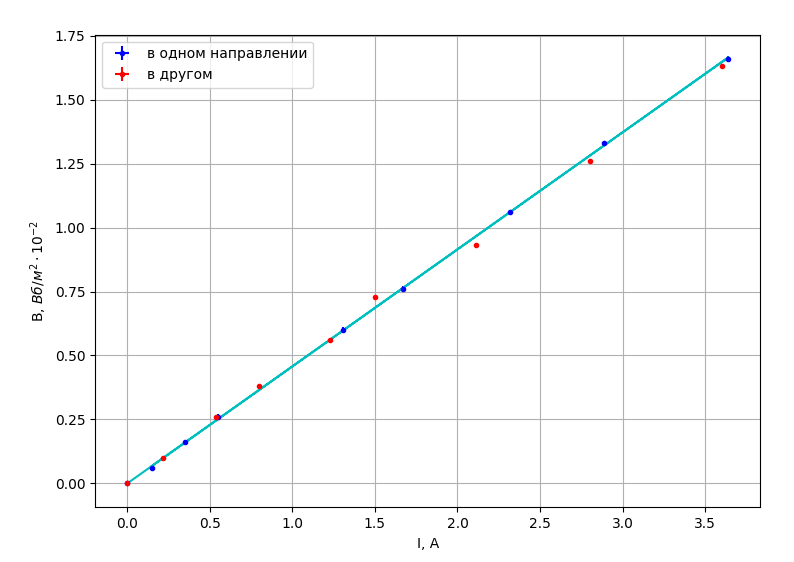
\includegraphics[width=0.65\linewidth]{Screenshot_4.png}
    \caption{Зависимость магнитного поля в соленоиде от тока в его обмотке}
\end{figure}

\subsubsection*{Определение фокусов}

Значение ускоряющего напряжения - $U_A = 960$ В

\begin{table}[h]
    \centering
    \begin{tabular}{|c|c|c|c|c|c|c|}
    \hline
         & \multicolumn{6}{|c|}{Первое направление тока} \\
    \hline
        номер фокуса & 1 & 2 & 3 & 4 & 5 & \\
    \hline
        I_{\text{ф}}, A & 0.64 & 1.3 & 1.96 & 2.61 & 3.35 & \\
    \hline
    \hline
         & \multicolumn{6}{|c|}{Противоположное направление тока} \\
    \hline
        номер фокуса & 1 & 2 & 3 & 4 & 5 & 6 \\
    \hline
        I_{\text{ф}}, A & 0.67 & 1.34 & 1.98 & 2.38 & 2.92 & 3.48\\
    \hline
    \end{tabular}
    \caption{Значения тока $I_\text{ф}$ в точках фокусов}
\end{table}

\subsubsection*{Определение значений $B_\text{ф}$}

\begin{table}[h]
    \centering
    \begin{tabular}{|c|c|c|c|c|c|c|}
    \hline
         номер фокуса & 1 & 2 & 3 & 4 & 5 & 6 \\
    \hline
        $B_\text{ф}$, $\frac{\text{Вб}}{\text{м}^2} \cdot 10^{-2}$ & 0.3 & 0.6 & 0.9 & 1.15 & 1.4 & 1.6\\
    \hline
    \end{tabular}
    \caption{Усреднённые значения $B_\text{ф}$}
\end{table}

\begin{figure}[h]
    \centering
    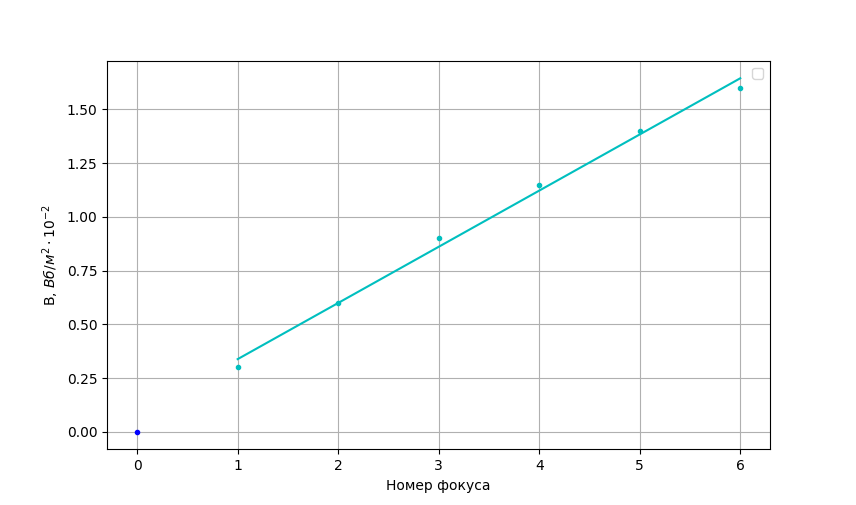
\includegraphics[width=0.65\linewidth]{Screenshot_5.png}
    \label{fig:placeholder}
\end{figure}

Наклон графика: 0,2614

$L = 0.265 м$

По формуле (2) и используя наклон графика и значение L определим удельный заряд электрона:

$e/m = 1.58*10^{11}$ Кл/кг

Табличное значение: $\frac{e}{m} = 1,76 \cdot 10^{11}$ Кл/кг

\newpage

\subsection*{Часть Б}

\subsubsection*{Характеристики приборов}
\begin{itemize}
    \item Миллиамперметр: $\Delta_{I_a} = 0,002$ мА (потому что стрелка чуть двигалась во время измерений);
    \item Амперметр соленоида: $\Delta_{I_m} = 0,004$ мА (потому что стрелка чуть двигалась во время измерений);
    \item Вольтметр: $\Delta_U = 0,5$ В;
    \item Параметр лампы k = $2,8 \cdot 10^{-2} \frac{T}{A}$;
    \item Параметр лампы $r_a$ = 12 мм.
\end{itemize}

\subsubsection*{Измерение зависимости анодного тока $I_A$ от тока через соленоид $I_C$}
Таблица со значениями $I_A$ и $I_C$ для разных значений напряжения $U_A$ приведена в конце отчёта.

\begin{figure}[h]
    \centering
    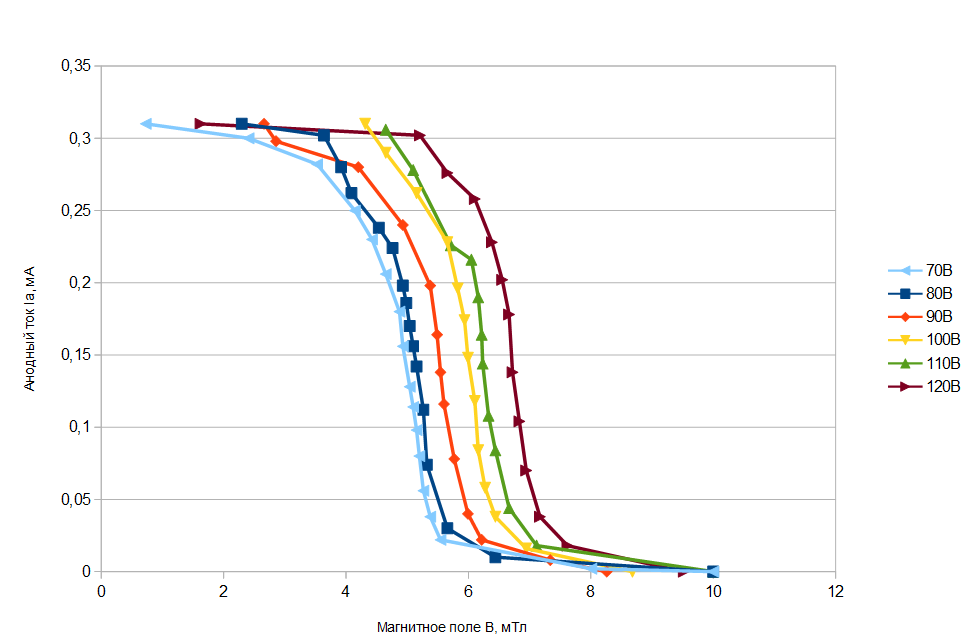
\includegraphics[width=0.75\linewidth]{Screenshot_6.png}
    \caption{Зависимость анодного тока $I_A$ от магнитного поля $B$}
    \label{fig:placeholder}
\end{figure}

По графику определяется $B_\text{кр}$:

\begin{table}[h]
    \centering
    \begin{tabular}{|c|c|c|c|c|c|c|}
    \hline
        $U_A$, В & 70 & 80 & 90 & 100 & 110 & 120 \\
    \hline
        $B_\text{кр}$, мТл & 4.94 & 5.12 & 5.52 & 5.98 & 6.23 & 6.75 \\
    \hline
    \end{tabular}
    \caption{Критичесие значения $B_\text{кр}$}
\end{table}

\begin{figure}[h]
    \centering
    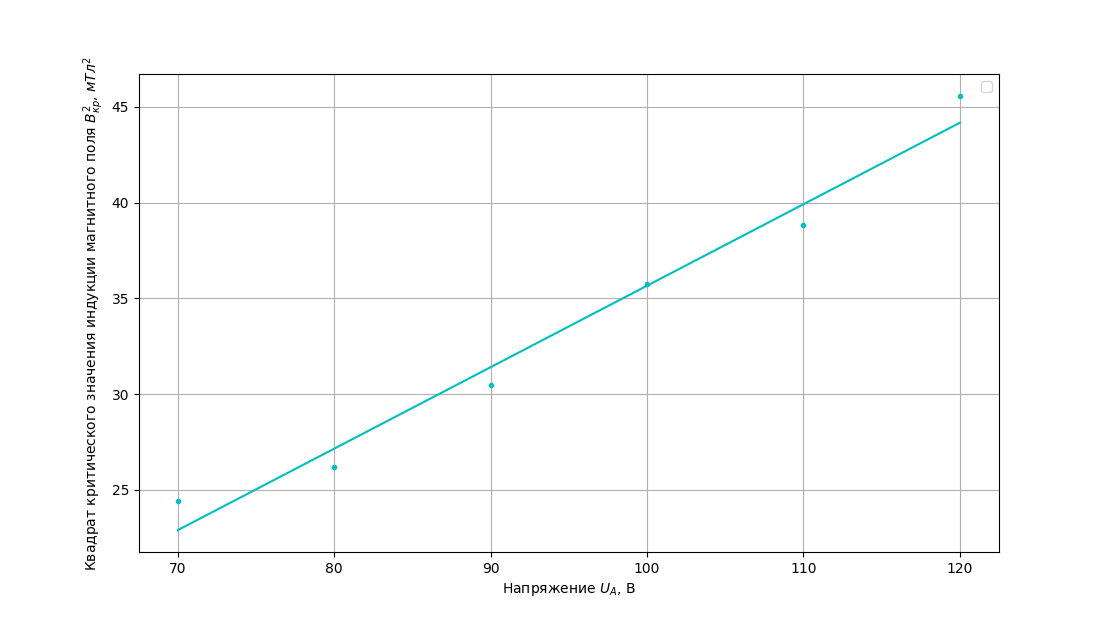
\includegraphics[width=0.5\linewidth]{Figure_1.png}
    \caption{Зависимость $B^2_\text{кр}$ от $U_A$}
    \label{fig:placeholder}
\end{figure}

Угловой коэффициент: 0.4254

По формуле (3) по угловому коэффициенту из графика определим заряд электрона $\frac{e}{m}$:
$$\frac{e}{m} = \frac{8}{0,4254 \cdot 12^2} = 1,306 \cdot 10^{11} \text{Кл/кг}$$

Табличное значение: $\frac{e}{m} = 1,76 \cdot 10^{11}$ Кл/кг

\newpage

\section*{Вывод}
Методом магнитной фокусировки: $e/m = (1,54 \pm 0,03)\cdot 10^{11}$ Кл/кг;

Методом магнетрона: $e/m = (1,29 \pm 0,09)\cdot 10^{11}$ Кл/кг.

Табличное значение удельного заряда $(e/m)_\text{теор} = 1,76\cdot 10^{11}$ Кл/кг. 

Оба метода дали результаты, сходящиеся по порядку с табличным значениием, однако первый метод (магнитной фокусировки) оказался точнее. Это можно объяснить низкой точностью миллиамперметра и определением $B_\text{кр}$ по графику.


\begin{table}[h]
\resizebox{\textwidth}{!}{%
\begin{tabular}{|lllllllllllllllllll|}
\hline
\multicolumn{19}{|l|}{\cellcolor[HTML]{C1F0C8}Напряжение $U_A$ = 70В}                                                                                                                               \\ \hline
\multicolumn{1}{|l|}{$I_M$, А}                       & 0,026 & 0,086 & 0,126 & 0,148 & 0,158 & 0,166 & 0,174 & 0,176 & 0,18  & 0,182 & 0,184 & 0,1856 & 0,188 & 0,192 & 0,198 & 0,286 & 0,6  & 0,9  \\
\multicolumn{1}{|l|}{$I_A$, мA}                      & 0,3   & 0,31  & 0,282 & 0,25  & 0,23  & 0,206 & 0,18  & 0,156 & 0,128 & 0,114 & 0,098 & 0,08   & 0,056 & 0,038 & 0,022 & 0,002 & 0    & 0    \\
\multicolumn{1}{|l|}{\cellcolor[HTML]{F7C7AC}B, мТл} & 0,728 & 2,408 & 3,528 & 4,144 & 4,424 & 4,648 & 4,872 & 4,928 & 5,04  & 5,096 & 5,152 & 5,1968 & 5,264 & 5,376 & 5,544 & 8,008 & 16,8 & 25,2 \\ \hline
\multicolumn{19}{|l|}{\cellcolor[HTML]{C1F0C8}Напряжение $U_A$ = 80В}                                                                                                                               \\ \hline
\multicolumn{1}{|l|}{$I_M$, А}                       & 0,082 & 0,13  & 0,14  & 0,146 & 0,162 & 0,17  & 0,176 & 0,178 & 0,18  & 0,182 & 0,184 & 0,188  & 0,19  & 0,202 & 0,23  & 0,7   &      &      \\
\multicolumn{1}{|l|}{$I_A$, мA}                      & 0,31  & 0,302 & 0,28  & 0,262 & 0,238 & 0,224 & 0,198 & 0,186 & 0,17  & 0,156 & 0,142 & 0,112  & 0,074 & 0,03  & 0,01  & 0     &      &      \\
\multicolumn{1}{|l|}{\cellcolor[HTML]{F7C7AC}B, мТл} & 2,296 & 3,64  & 3,92  & 4,088 & 4,536 & 4,76  & 4,928 & 4,984 & 5,04  & 5,096 & 5,152 & 5,264  & 5,32  & 5,656 & 6,44  & 19,6  &      &      \\ \hline
\multicolumn{19}{|l|}{\cellcolor[HTML]{C1F0C8}Напряжение $U_A$ = 90В}                                                                                                                               \\ \hline
\multicolumn{1}{|l|}{$I_M$, А}                       & 0,095 & 0,102 & 0,15  & 0,176 & 0,192 & 0,196 & 0,198 & 0,2   & 0,206 & 0,214 & 0,222 & 0,262  & 0,295 &       &       &       &      &      \\
\multicolumn{1}{|l|}{$I_A$, мA}                      & 0,31  & 0,298 & 0,28  & 0,24  & 0,198 & 0,164 & 0,138 & 0,116 & 0,078 & 0,04  & 0,022 & 0,008  & 0     &       &       &       &      &      \\
\multicolumn{1}{|l|}{\cellcolor[HTML]{F7C7AC}B, мТл} & 2,66  & 2,856 & 4,2   & 4,928 & 5,376 & 5,488 & 5,544 & 5,6   & 5,768 & 5,992 & 6,216 & 7,336  & 8,26  &       &       &       &      &      \\ \hline
\multicolumn{19}{|l|}{\cellcolor[HTML]{C1F0C8}Напряжение $U_A$ = 100В}                                                                                                                              \\ \hline
\multicolumn{1}{|l|}{$I_M$, А}                       & 0,154 & 0,166 & 0,184 & 0,202 & 0,208 & 0,212 & 0,214 & 0,218 & 0,222 & 0,224 & 0,23  & 0,248  & 0,31  &       &       &       &      &      \\
\multicolumn{1}{|l|}{$I_A$, мA}                      & 0,31  & 0,29  & 0,262 & 0,228 & 0,196 & 0,174 & 0,148 & 0,118 & 0,084 & 0,058 & 0,038 & 0,016  & 0     &       &       &       &      &      \\
\multicolumn{1}{|l|}{\cellcolor[HTML]{F7C7AC}B, мТл} & 4,312 & 4,648 & 5,152 & 5,656 & 5,824 & 5,936 & 5,992 & 6,104 & 6,216 & 6,272 & 6,44  & 6,944  & 8,68  &       &       &       &      &      \\ \hline
\multicolumn{19}{|l|}{\cellcolor[HTML]{C1F0C8}Напряжение $U_A$ = 110В}                                                                                                                              \\ \hline
\multicolumn{1}{|l|}{$I_M$, А}                       & 0,166 & 0,182 & 0,204 & 0,216 & 0,22  & 0,222 & 0,224 & 0,226 & 0,23  & 0,238 & 0,254 & 0,55   &       &       &       &       &      &      \\
\multicolumn{1}{|l|}{$I_A$, мA}                      & 0,306 & 0,278 & 0,226 & 0,216 & 0,19  & 0,164 & 0,144 & 0,108 & 0,084 & 0,044 & 0,018 & 0      &       &       &       &       &      &      \\
\multicolumn{1}{|l|}{\cellcolor[HTML]{F7C7AC}B, мТл} & 4,648 & 5,096 & 5,712 & 6,048 & 6,16  & 6,216 & 6,272 & 6,328 & 6,44  & 6,664 & 7,112 & 15,4   &       &       &       &       &      &      \\ \hline
\multicolumn{19}{|l|}{\cellcolor[HTML]{C1F0C8}Напряжение $U_A$ = 120В}                                                                                                                              \\ \hline
\multicolumn{1}{|l|}{$I_M$, А}                       & 0,058 & 0,186 & 0,202 & 0,218 & 0,228 & 0,234 & 0,238 & 0,24  & 0,244 & 0,248 & 0,256 & 0,272  & 0,34  &       &       &       &      &      \\
\multicolumn{1}{|l|}{$I_A$, мA}                      & 0,31  & 0,302 & 0,276 & 0,258 & 0,228 & 0,202 & 0,178 & 0,138 & 0,104 & 0,07  & 0,038 & 0,018  & 0     &       &       &       &      &      \\
\cellcolor[HTML]{F7C7AC}B, мТл                       & 1,624 & 5,208 & 5,656 & 6,104 & 6,384 & 6,552 & 6,664 & 6,72  & 6,832 & 6,944 & 7,168 & 7,616  & 9,52  &       &       &       &      &      \\ \hline
\end{tabular}%
}
\end{table}


\end{document}
